% Requires graphicx. Compile from Manuscript/. All four diagrams derive from coded records.
\begin{figure*}[t]
\centering
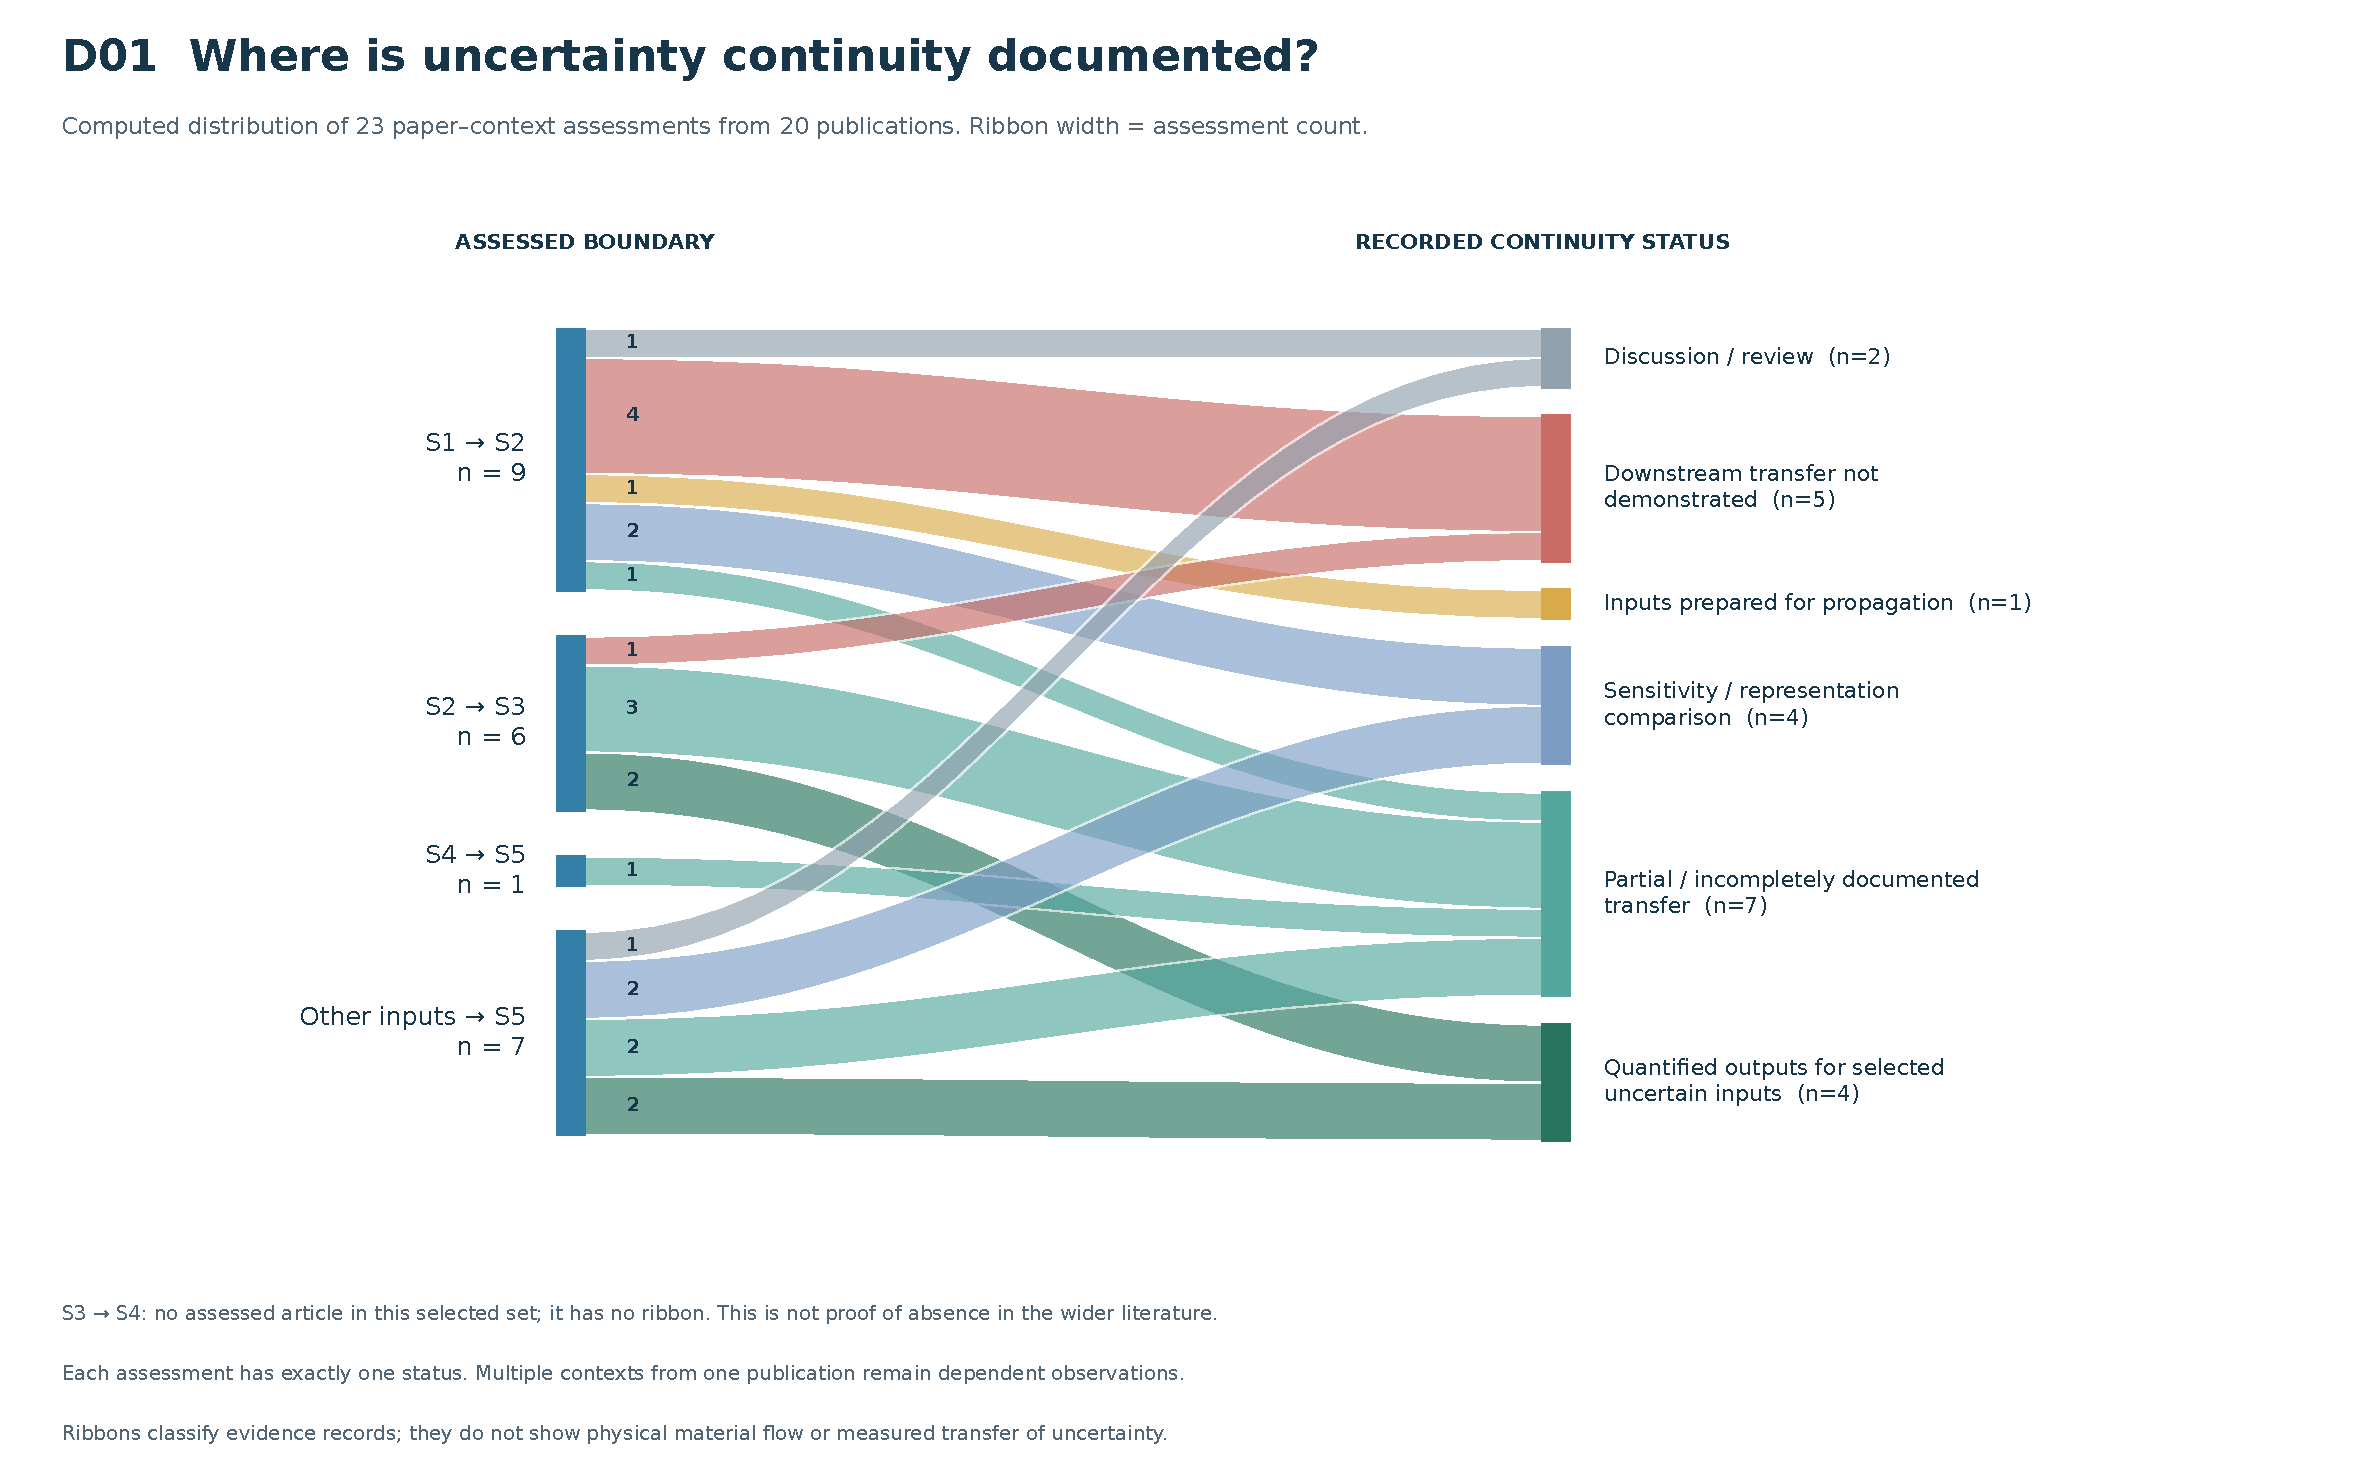
\includegraphics[width=\textwidth]{relational_analysis/data_diagrams/figures/D01_boundary_continuity_alluvial.pdf}
\caption{Distribution of 23 publication--context assessments across material-flow boundaries and recorded uncertainty-continuity categories. Ribbon widths equal assessment counts. Ribbons classify evidence; they are not measured material or uncertainty flows.}
\label{fig:data-continuity}
\end{figure*}

\begin{figure*}[t]
\centering
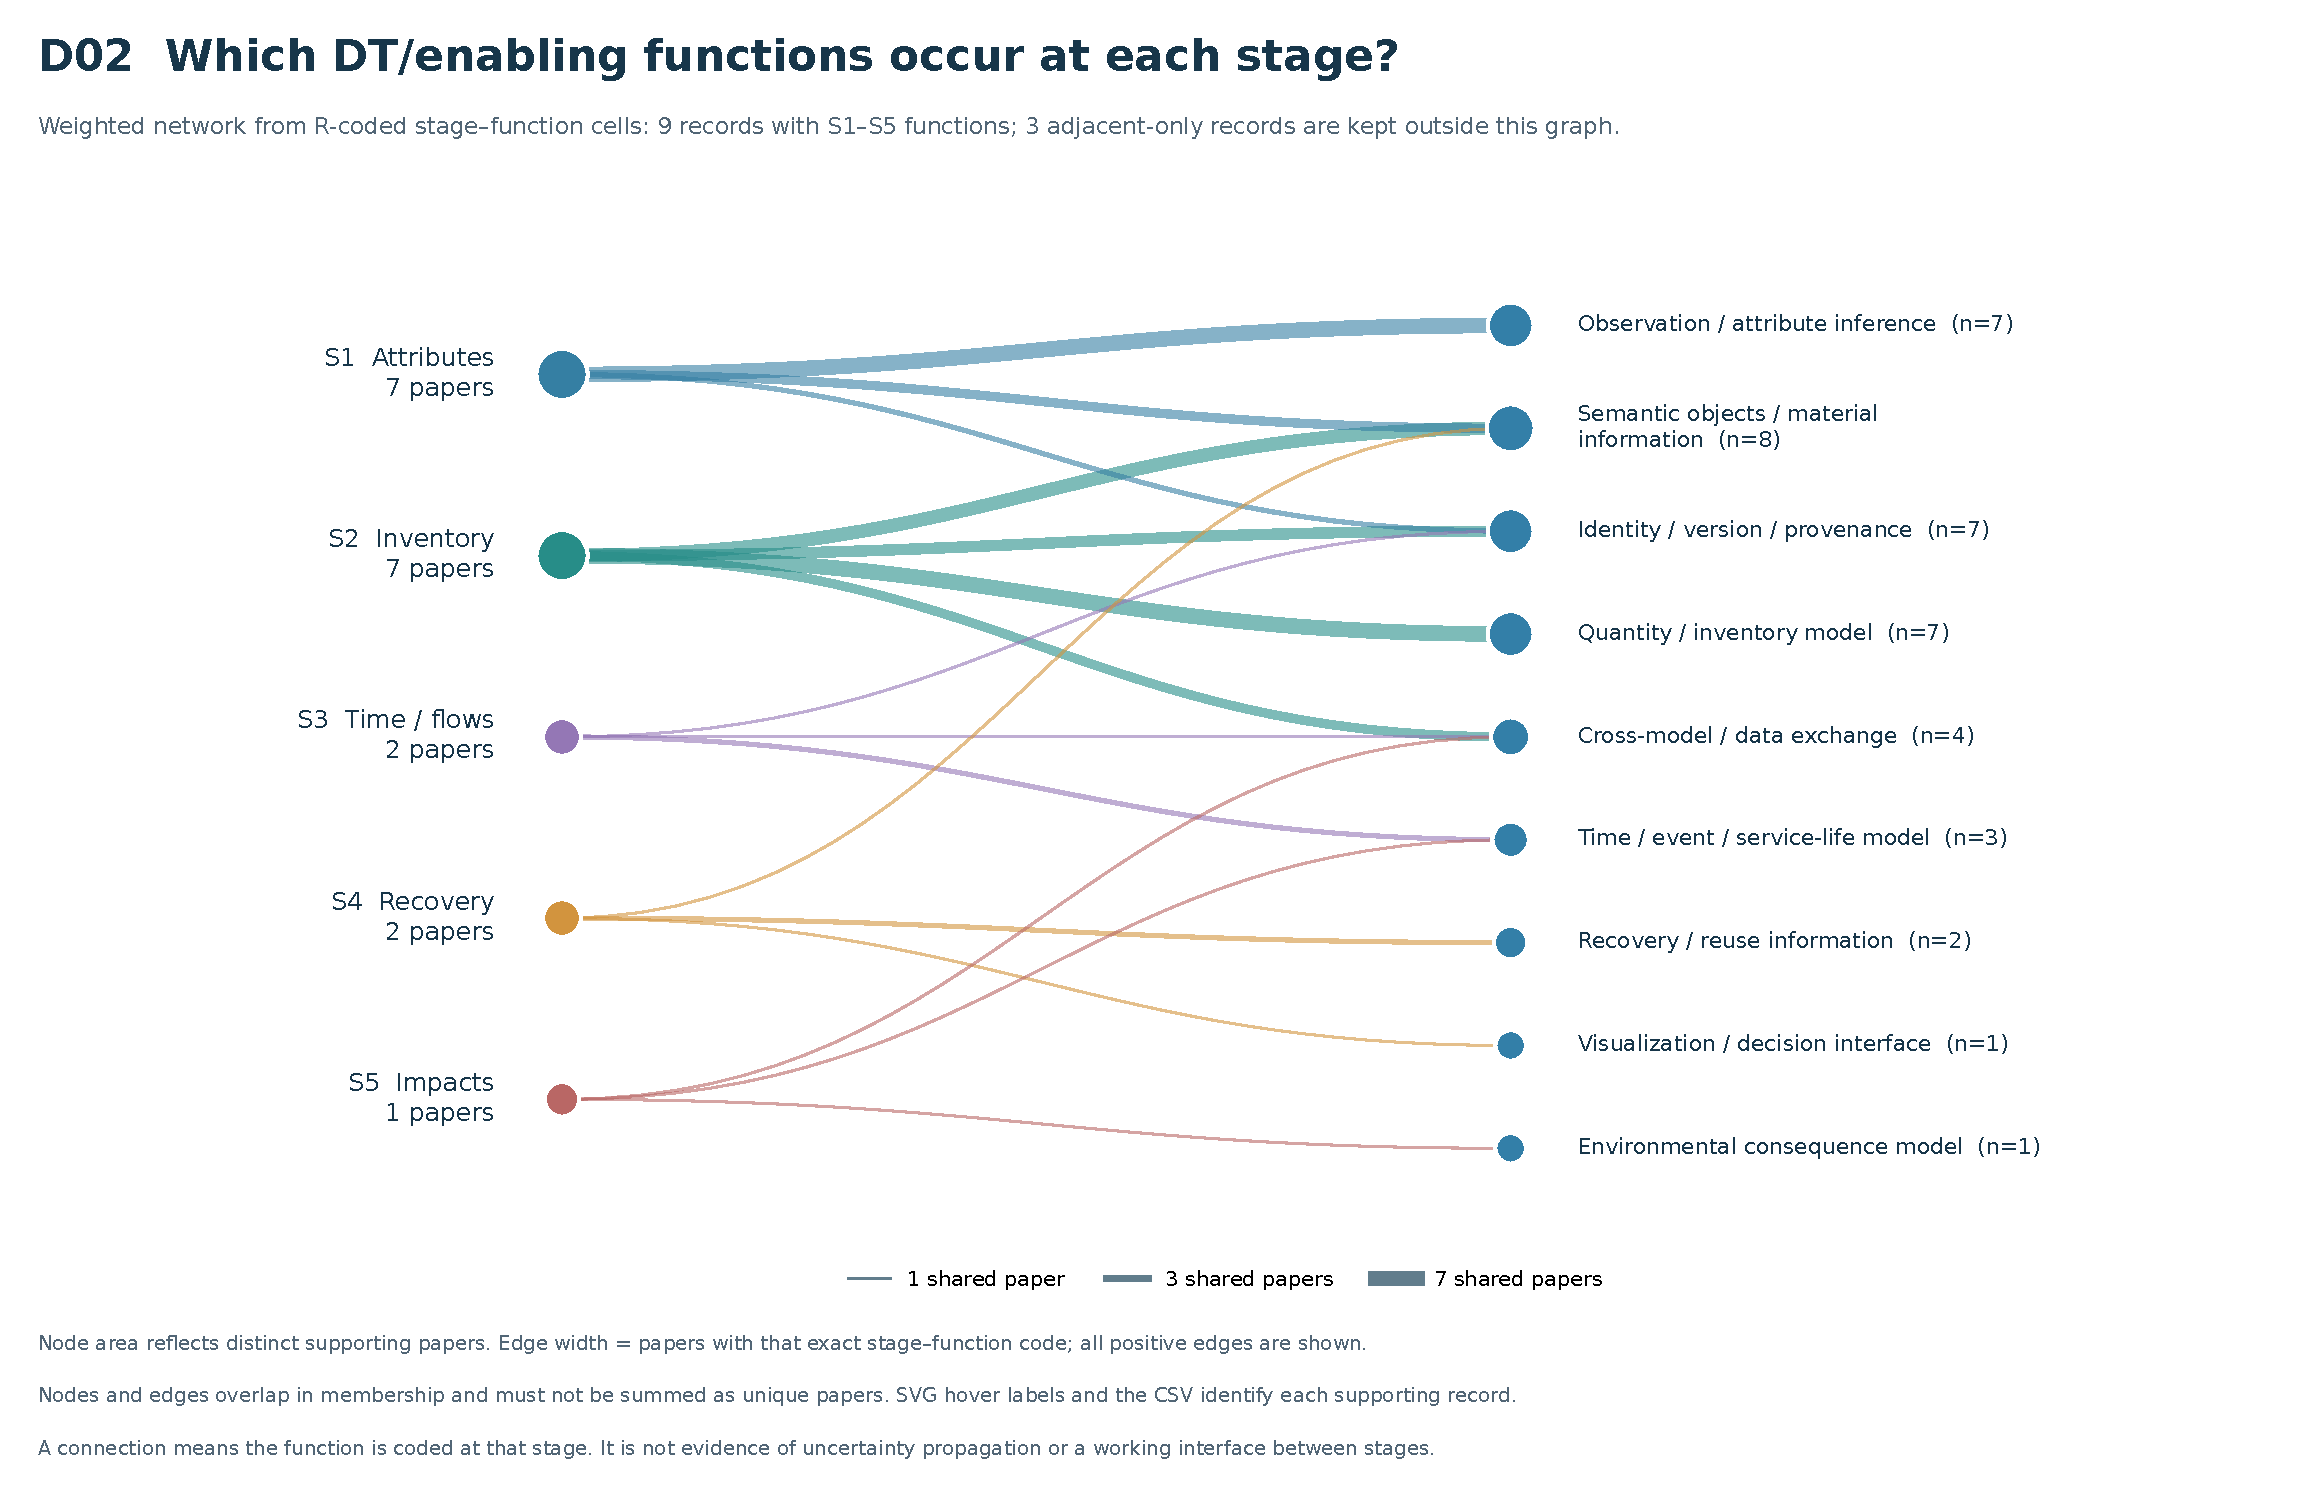
\includegraphics[width=\textwidth]{relational_analysis/data_diagrams/figures/D02_stage_function_network.pdf}
\caption{Weighted stage--function incidence network calculated from nine publications with R-coded functions in S1--S5. All 16 positive edges are shown; edge width is the distinct-publication count for the pair. Three adjacent-only records are excluded. The graph does not establish directed interfaces or uncertainty transport.}
\label{fig:data-stage-network}
\end{figure*}

\begin{figure*}[t]
\centering
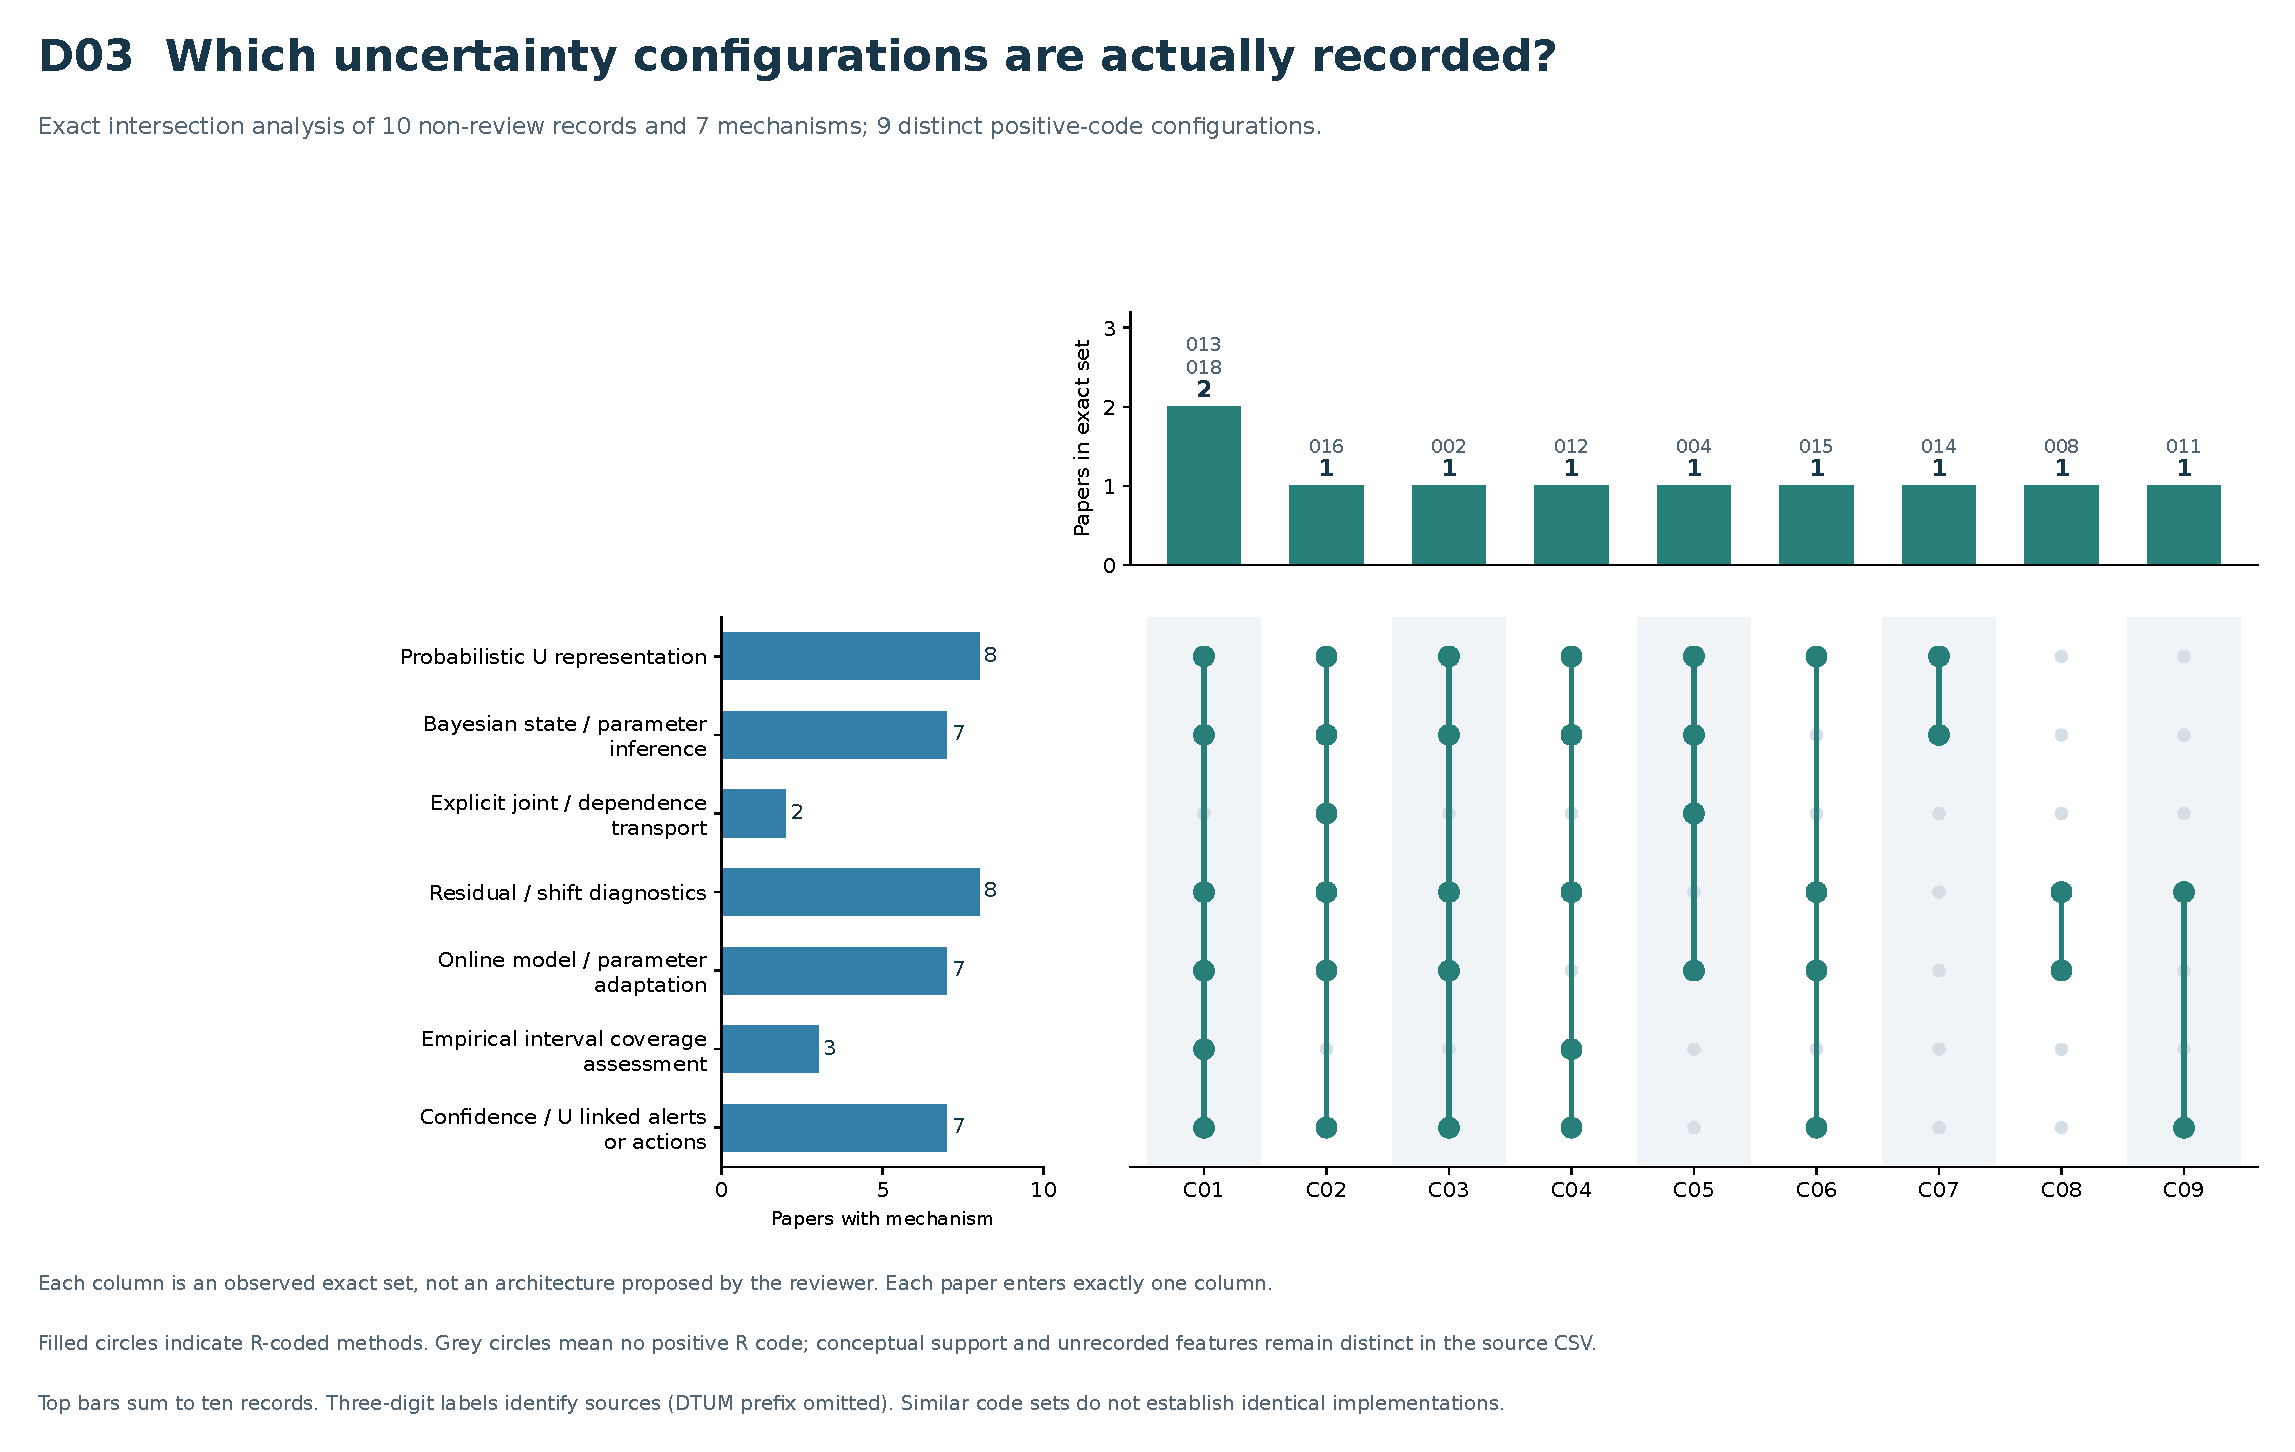
\includegraphics[width=\textwidth]{relational_analysis/data_diagrams/figures/D03_exact_uncertainty_configurations.pdf}
\caption{Exact positive-code configurations of seven uncertainty mechanisms among ten non-review records. Each record enters one configuration, yielding nine distinct sets. Filled dots identify described methods; grey dots indicate no positive R code. The columns are observed code sets, not predefined or validated architecture classes.}
\label{fig:data-configurations}
\end{figure*}

\begin{figure*}[t]
\centering
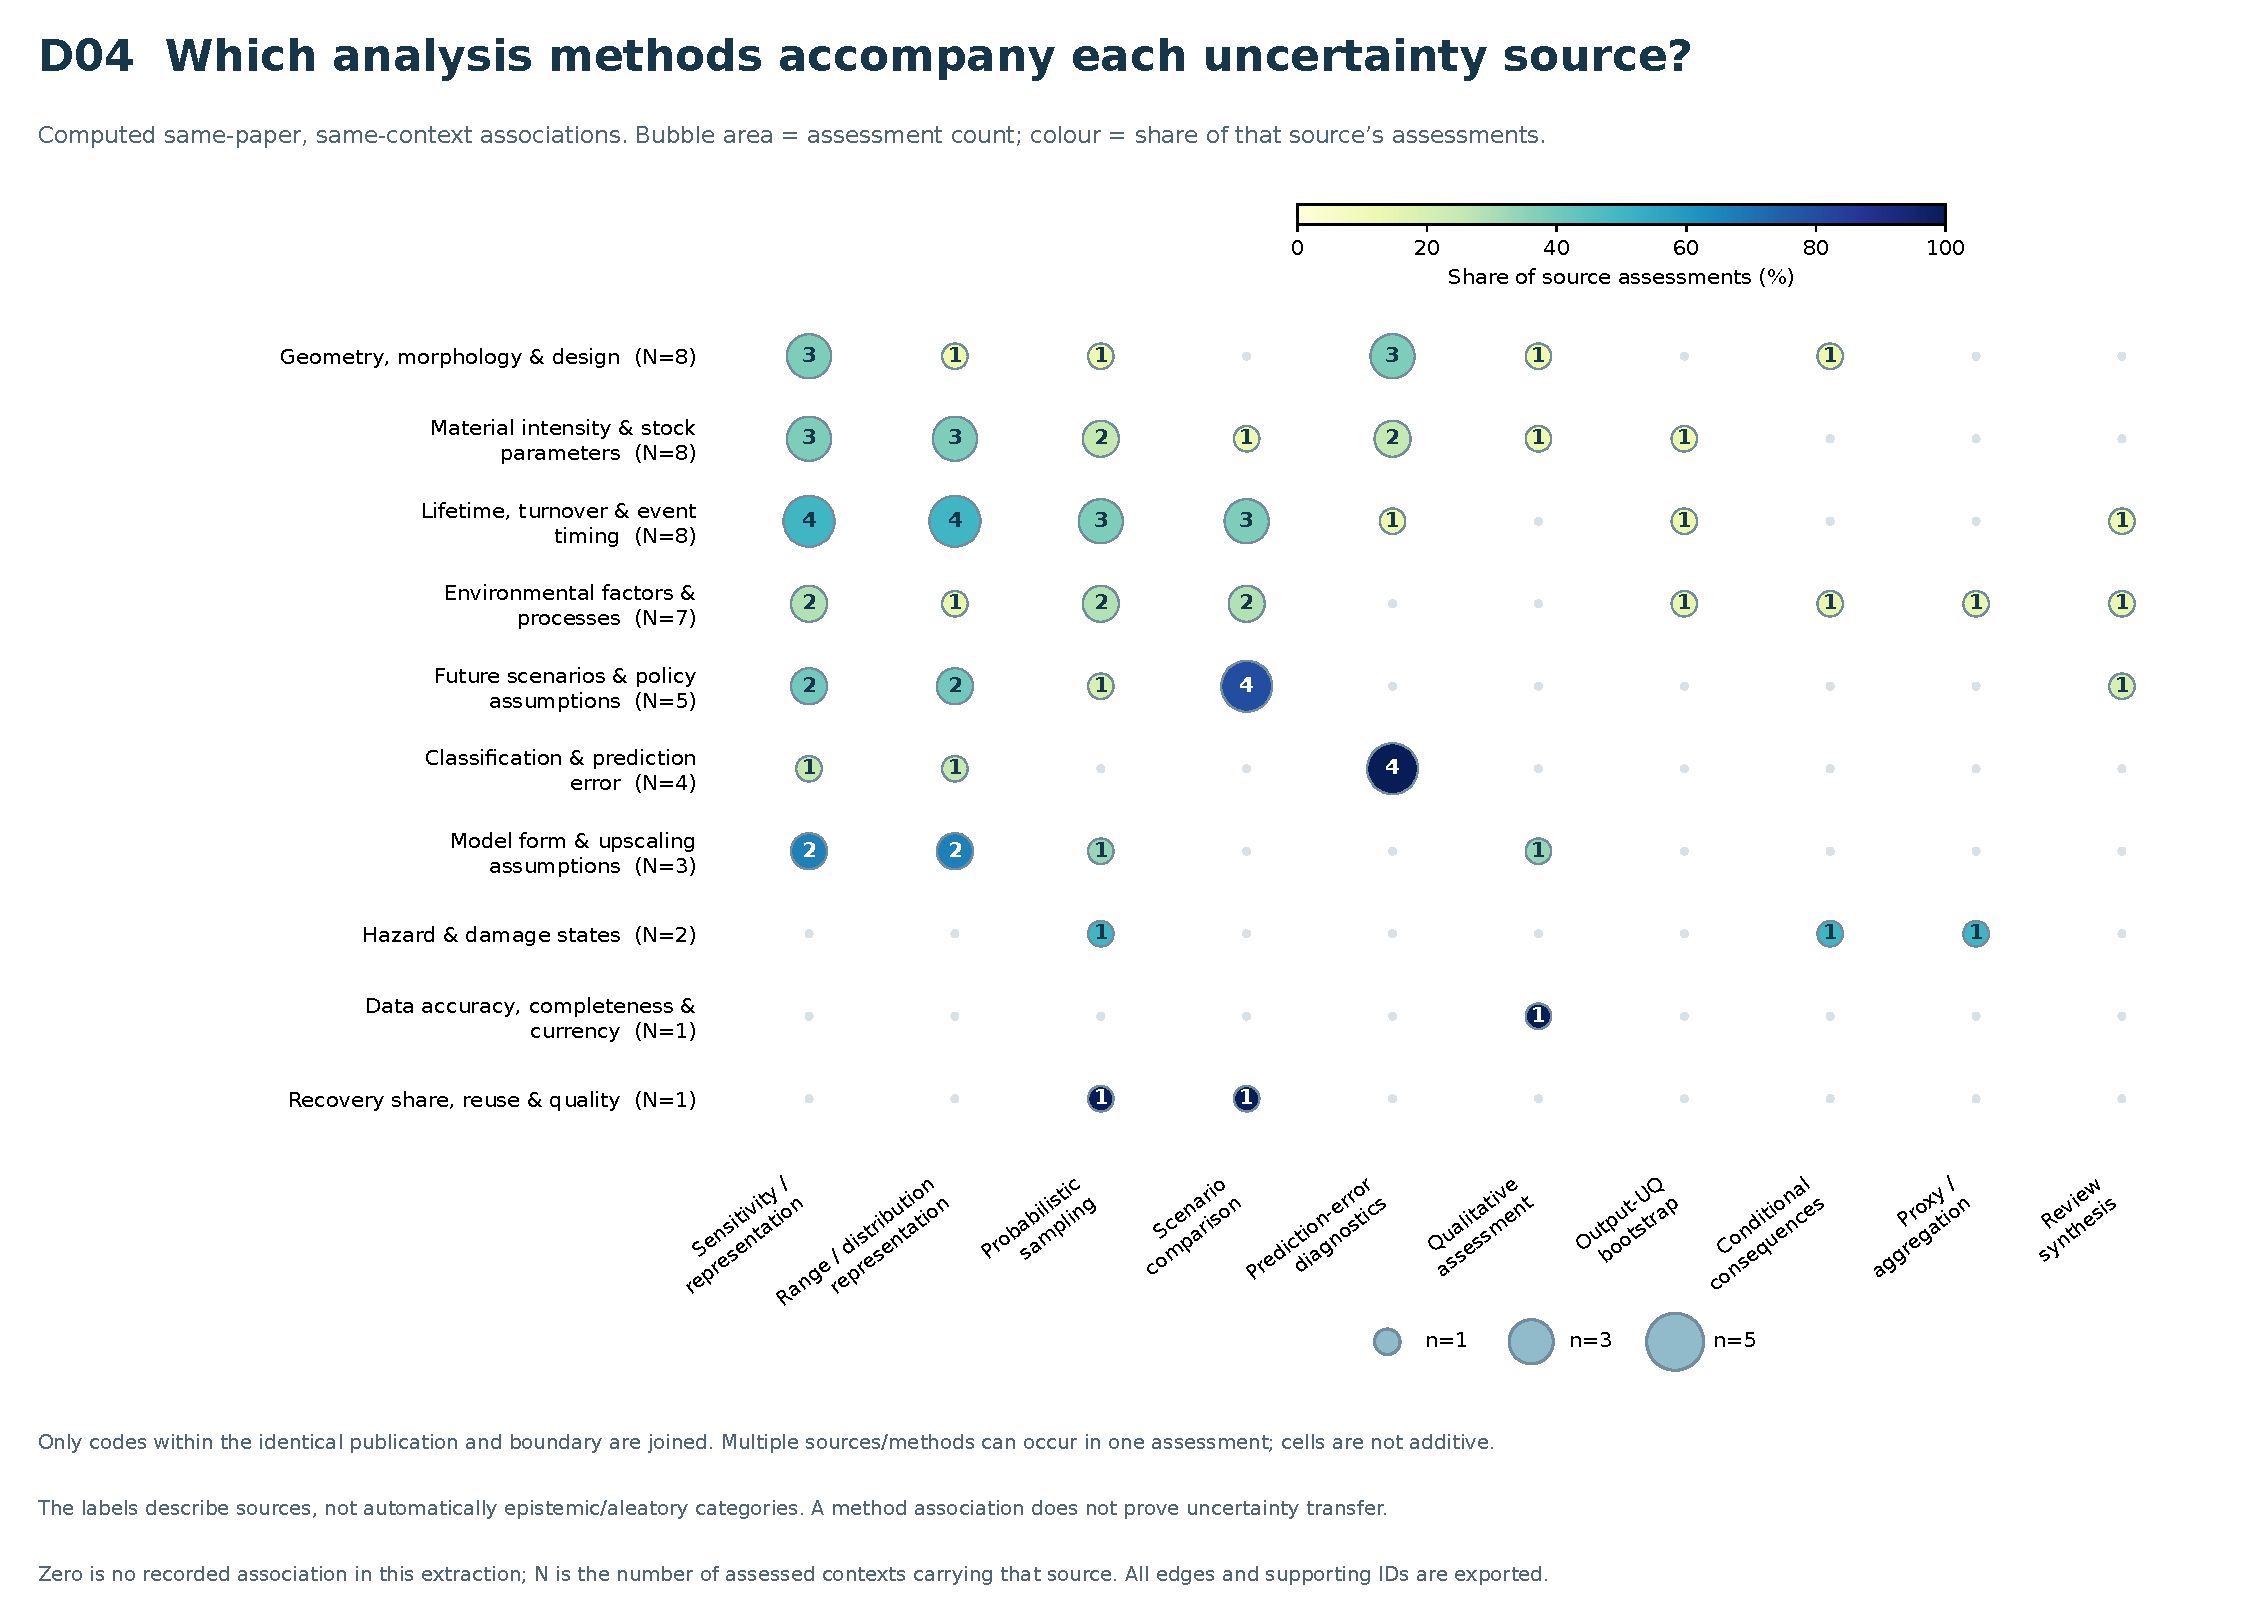
\includegraphics[width=\textwidth]{relational_analysis/data_diagrams/figures/D04_uncertainty_source_method_associations.pdf}
\caption{Co-occurrence of uncertainty sources and analysis methods within the identical publication and material-flow context. Bubble area gives the assessment count and colour the share of assessments carrying the source. The 46 positive pairs are descriptive associations, not causal or propagation claims.}
\label{fig:data-source-method}
\end{figure*}
